\section{Implementation}
\label{sec:imp}

This section presents the implementation of our stepper.  We step-evaluate programs in the following way.
First, we convert a given program into an abstract syntax tree using the built-in parser of OCaml.
Next, we pass the parsed program to a stepping interpreter,
which outputs the whole program at each reduction step.
The output programs are then processed by an Emacs Lisp program,
in such a way that the user can see the steps one by one.  Here we focus our attention to the stepping interpreter,
which plays the key role in the whole stepping system.

As the stepper is supposed to tell us how a program is evaluated, we have to make sure that it evaluates programs in the same order as the OCaml interpreter does.
For the presentation issue, here we restrict ourselves to a toy language,
consisting of lambda terms and a simplified version of the try-with construct.
The full language supported by the current stepper is presented in Section \ref{sec:imp:ocaml}.  

\subsection{Building an Interpreter}
\label{sec:imp:interpreter}

\begin{figure}
\begin{verbatim}
type e_t = Var of string               (* x *)
         | Fun of string * e_t         (* fun x -> e *)
         | App of e_t * e_t            (* e e *)
         | Try of e_t * string * e_t   (* try e with x -> e *)
         | Raise of e_t                (* raise e *)
\end{verbatim}
\caption{Syntax}
\label{figure:typee}
\end{figure}

\begin{figure}
\begin{verbatim}
(* exception holding the value of input program's exception *)
exception Error of e_t

(* evaluate expression *)
(* eval : e_t -> e_t *)
let rec eval expr = match expr with
  | Var (x) -> failwith ("unbound variable: " ^ x)
  | Fun (x, e) -> Fun (x, e)
  | App (e1, e2) ->
    begin
      let v2 = eval e2 in
      let v1 = eval e1 in
      match v1 with
      | Fun (x, e) ->
        let e' = subst e x v2 in   (* substitute v2 for x in e *)
        let v = eval e' in
        v
      | _ -> failwith "not a function"
    end
  | Try (e1, x, e2) ->
    begin
      try
        let v1 = eval e1 in
        v1
      with Error (v) ->
        let e2' = subst e2 x v in   (* substitute v for x in e2 *)
        eval e2'
    end
  | Raise (e) ->
    let v = eval e in
    raise (Error (v))

(* start evaluation *)
(* start : e_t -> e_t *)
let start e =
  try
    eval e
  with
    Error v -> Raise v
\end{verbatim}
\caption{Big-step interpreter}
\label{figure:interpreter}
\end{figure}

In Figures \ref{figure:typee} and \ref{figure:interpreter},
we define the object language as well as a big-step interpreter.
The \texttt{eval} function evaluates a given expression following OCaml's call-by-value, right-to-left strategy.
For instance, when given an application \texttt{e1 e2},
it first evaluates the argument \texttt{e2}, then evaluates the function \texttt{e1}.
Once the application has been turned into a redex, we perform $\beta$-reduction, and evaluate the post-reduction expression.
Note that, when the top-level expression is an executable, closed program, the input of the \texttt{eval} function cannot be a variable.  The reason is that we never touch a function's body before it receives an argument, and that $\beta$-reduction replaces lambda-bound variables with values.

Object-level exception handling is performed by the meta-level \texttt{try} and \texttt{raise} constructs.
Specifically, when evaluating \texttt{raise e},
we first evaluate \texttt{e} to some value \texttt{v},
and then raise a meta-level (OCaml) exception \texttt{Error v}.
If an exception \texttt{Error v} was raised during evaluation of \texttt{e1} in \texttt{try e1 with x -> e2}, the \texttt{eval} function ignores the rest of the computation in \texttt{e1}, and evaluates \texttt{e2} with \texttt{v} substituted for \texttt{x}.  This is exactly how OCaml's try-with construct works.  For convenience, we will hereafter call \texttt{e1} a \emph{tryee}; the intention is that \texttt{e1} is the expression being ``tried'' by the handler.   

The main function \texttt{start} calls \texttt{eval} in an exception handling context.  From the construction, we can see that any expression that has a \texttt{raise e} with no matching \texttt{try} clause will be evaluated to \texttt{raise v}.  For example, \texttt{2 + 3 + (raise 4) + 5} evaluates to \texttt{raise 4}.

\subsection{Turning the Interpreter into a Stepper}
\label{sec:imp:stepper}

As stated in Section \ref{sec:intro}, a stepper must display the whole program at each reduction step.  Consider the simple arithmetic expression \texttt{(1 + 2 * 3) + 4}.  When step-executing this expression, we want to see the following reduction sequence:
\[
\begin{array}{cl}
            & \mathtt{(1 + 2 * 3) + 4} \\
\rightarrow & \mathtt{(1 + 6) + 4} \\
\rightarrow & \mathtt{7 + 4} \\
\rightarrow & \mathtt{11}
\end{array}
\]

The interpreter in Figure \ref{figure:interpreter}, however, does not immediately give us these steps.  Suppose the \texttt{eval} function is evaluating the subexpression \texttt{2 * 3}.  We can display this subexpression using a printing function, but we do not have enough information to reconstruct the whole program.  What is missing here is the \emph{context} surrounding \texttt{2 * 3}, namely \texttt{(1 + [.])\ + 4} (where \texttt{[.]} denotes the hole of the context).  Hence, to implement a stepper, we need to keep track of every evaluation context we have traversed.  

In Figure \ref{figure:simpleplug}, we define context frames as algebraic data of type \texttt{frame\_t}.  Each frame represents evaluation of some subexpression: \eg, \texttt{CAppR (e1)} tells us that we are evaluating the argument part of an application, whose function part is \texttt{e1}.  Evaluation contexts are defined as lists of these frames (spoiler alert: this does not work for exceptions).  We then define the \texttt{plug} function, which reconstructs a program by wrapping the expression \texttt{expr} with context frames in \texttt{ctxt}. 

\begin{figure}
\begin{verbatim}
(* context frames *)
type frame_t = 
             | CAppR of e_t           (* e [.] *)
             | CAppL of e_t           (* [.] v  *)
             | CTry of string * e_t   (* try [.] with x -> e *)
             | CRaise                 (* raise [.] *)

(* evaluation contexts *)
type c_t = frame_t list

(* reconstruct the whole program *)
(* plug : e_t -> c_t -> e_t *)
let rec plug expr ctxt = match ctxt with
  | [] -> expr
  | CAppR (e1) :: rest -> plug (App (e1, expr)) rest
  | CAppL (e2) :: rest -> plug (App (expr, e2)) rest
  | CTry (x, e2) :: rest -> plug (Try (expr, x, e2)) rest
  | CRaise :: rest -> plug (Raise expr) rest
\end{verbatim}
\caption{Contexts and reconstruction function; first attempt}
\label{figure:simpleplug}
\end{figure}

Now, if we let the evaluation function receive an additional argument representing the context, we should be able to display all the steps of the arithmetic expression \texttt{(1 + 2 * 3) + 4}.  For instance, when evaluating the subexpression \texttt{2 * 3}, the extra argument will be a two-element list \texttt{[(1 + [.]);\ ([.]\ + 4)]}, and we can obtain the whole program using the \texttt{plug} function.

The resulting stepper is essentially the CK abstract machine
\cite{FF1986}, where the expression is the control string and the
evaluation context is the continuation.
Substitution is used to implement $\beta$-reduction.
We did not implement the abstract machine directly but augmented a
big-step interpreter, because we want to keep the correspondence between
big-step execution and small-step execution.
It enables us to skip evaluation of user-specified function application,
as we elaborate in Section~\ref{sec:imp:ocaml}.

Unfortunately, this na\"ive implementation does not work in the presence of exception handlers.  Consider \texttt{try (2 + 3 * (raise 4) + 5) with x -> x}.  When step-executing this expression, we expect to see the following steps:

\vspace{0.2cm}

\noindent \texttt{(* Step 0 *) try (\colorbox{lightgreen}{2 + (3 * (raise 4)) + 5}) with x -> x\\
  (* Step 1 *) try (\colorbox{purple}{raise 4}) with x -> x\\
  (* Step 1 *) \colorbox{lightgreen}{try (raise 4) with x -> x}\\
  (* Step 2 *) \colorbox{purple}{4}\\
}

\vspace{0.2cm}

\noindent The first reduction happens when the input to the stepping interpreter is \texttt{raise 4}.  However, observe that the highlighted redex is a bigger expression \texttt{(2 + 3 * (raise 4) + 5)}, because reduction of a \texttt{raise} construct discards the context \emph{within} the tryee.  Since context frames are collected in a single list, the second argument at this point will be \texttt{[(3 * [.]); (2 + [.]);\ ([.]\ + 5);\ (try [.]\ with x -> x)]}, \ie, it contains the context \emph{outside} the tryee.  This suggests that, when dealing with exception handlers, we have to distinguish between contexts inside and outside a tryee.\footnote{
The destination is not necessary,
if we want to support only exception handling.
We could simply search for the enclosing handler in the evaluation
context.
However, it requires a linear search through the evaluation context.
Furthermore, distinction is necessary if we want to implement
more general control operators,
such as shift and reset \cite{DF1990}.
}

\begin{figure}
\begin{verbatim}
(* frames *)
type frame_t = 
             | CAppR of e_t          (* e [.] *)
             | CAppL of e_t          (* [.] v *)
             | CRaise                (* raise [.] *)

(* try frame *)
type ctry_t = 
            | CHole                        (* [.] *)
            | CTry of string * e_t * c_t   (* try [.] with x -> e *)

(* evaluation context *)
and c_t = frame_t list * ctry_t

(* reconstruct tryee *)
(* plug_in_try : e_t -> frame_t list -> e_t *)
let rec plug_in_try expr ctxt = match ctxt with
  | [] -> expr
  | first :: rest -> match first with
    | CAppR (e1) -> plug_in_try (App (e1, expr)) rest
    | CAppL (e2) -> plug_in_try (App (expr, e2)) rest
    | CRaise -> plug_in_try (Raise (expr)) rest

(* reconstruct the whole program *)
(* plug : e_t -> c_t -> e_t *)
let rec plug expr (clist, tries) =
  let tryee = plug_in_try expr clist in
  match tries with
  | CHole -> tryee
  | CTry (x, e2, outer) -> plug (Try (tryee, x, e2)) outer
\end{verbatim}
  \caption{Contexts and reconstruction function; final version}
  \label{figure:typec}
\end{figure}

In Figure \ref{figure:typec}, we present a refined definition of evaluation contexts.  We see a new definition of context frames \texttt{frame\_t}, where \texttt{CTry} is missing.  When evaluating a program that uses try-with constructs, these frames are used to build a delimited context within a tryee.  We next find a separate datatype \texttt{ctry\_t}, which can be understood as meta contexts.  Then we define evaluation contexts as pairs of delimited and meta contexts.  As an example, when evaluating \texttt{raise 4} in the following expression:
\begin{verbatim}
0 + (try 1 + 2 * (try (3 + raise 4) - 5 with x -> x + 6) with y -> y)
\end{verbatim}
\noindent the current context looks like:
\begin{verbatim}
([(3 + [.]); ([.] - 5)],
  CTry ("x", x + 6,
    ([2 * [.]; 1 + [.]],
      CTry ("y", y,
        ([0 + [.]], CHole)))))
\end{verbatim}

The refined contexts allow us to first reconstruct the expression up to the tryee using the \texttt{frame\_t} contexts, and then build up the whole program using the \texttt{ctry\_t} contexts.  In our particular example, the stepper reconstructs \texttt{(3 + raise 4) - 5}, highlights it, and reconstructs the whole program.

To give the reader a better idea how context frames are accumulated, let us demonstrate the evaluation of an expression involving exception handling:

\begin{verbatim}
eval (2 * (try 3 + (raise 4) - 5 with x -> x + 6)) ([], CHole)
eval (try 3 + (raise 4) - 5 with x -> x + 6) ([2 * [.]], CHole)
eval (3 + (raise 4) - 5) ([], CTry ("x", x + 6, ([2 * [.]], CHole)))
eval 5 ([3 + (raise 4) - [.]], CTry ("x", x + 6, ([2 * [.]], CHole)))
eval (3 + (raise 4)) ([[.] - 5], CTry ("x", x + 6, ([2 * [.]], CHole)))
eval (raise 4) ([3 + [.]; [.] - 5], CTry ("x", x + 6, ([2 * [.]], CHole)))
eval 4 ([raise [.]; 3 + [.]; [.] - 5], CTry ("x", x + 6, ([2 * [.]], CHole)))
eval (4 + 6) ([2 * [.]], CHole)
\end{verbatim}

\noindent Observe that we discard the context within the tryee, namely \texttt{3 + (raise [.])\ - 5}, at the last step.

Now we present our stepping interpreter in Figure \ref{figure:stepper}.  The function extends the big-step interpreter in two ways (as shaded in the figure): (i) it receives an argument representing the evaluation context; and (ii) it outputs the current program every time reduction takes place.  

\begin{figure}
%(* add a non-try frame *)
%(* add : c_t -> frame_t -> c_t *)
%let rec add (list, outer) ctxt = (ctxt :: list, outer)
%
%(* add a try frame *)
%(* add_try : c_t -> string -> e_t -> c_t *)
%let rec add_try ctxt var expr = ([], CTry (var, expr, ctxt))  

\begin{alltt}
(* stepping evaluator *)
(* eval : e_t -> c_t -> e_t *)
let rec eval expr \colorbox{lightgray}{ctxt} = match expr with       (* add an argument for context *)
  | Var (x) -> failwith ("unbound variable: " ^ x)
  | Lam (x, e) -> Lam (x, e)
  | App (e1, e2) ->
    begin
      let v2 = eval e2 \colorbox{lightgray}{(add ctxt (CAppR e1))} in           (* add context info *)
      let v1 = eval e1 \colorbox{lightgray}{(add ctxt (CAppL v2))} in           (* add context info *)
      match v1 with
      | Lam (x, e) ->
        let e' = subst e x v2 in
        \colorbox{lightgray}{memo (App (v1, v2)) e' ctxt;}                       (* output programs *)
        let v = eval e' \colorbox{lightgray}{ctxt} in                           (* add context info *)
        v
      | _ -> failwith "not a function"
    end
  | Try (e1, x, e2) ->
    begin
      try
        let v1 = eval e1 \colorbox{lightgray}{(add_try ctxt x e2)} in           (* add context info *)
        \colorbox{lightgray}{memo (Try (v1, x, e2)) v1 ctxt;}                    (* output programs *)
        v1
      with Error (v) ->
        let e2' = subst e2 x v in
        \colorbox{lightgray}{memo (Try (Raise v, x, e2)) e2' ctxt;}              (* output programs *)
        eval e2' \colorbox{lightgray}{ctxt}                                     (* add context info *)
    end
  | Raise (e0) ->
    let v = eval e0 \colorbox{lightgray}{(add ctxt CRaise)} in                  (* add context info *)
    \colorbox{lightgray}{begin match ctxt with                   }
\end{alltt}
\vspace{-18pt}
\begin{alltt}
    \colorbox{lightgray}{    | ([], _) -> ()                     }
\end{alltt}
\vspace{-18pt}
\begin{alltt}
    \colorbox{lightgray}{    | (clist, tries) ->                 }
\end{alltt}
\vspace{-18pt}
\begin{alltt}
    \colorbox{lightgray}{      memo (plug_in_try (Raise v) clist)}               (* output programs *)
\end{alltt}
\vspace{-18pt}
\begin{alltt}
    \colorbox{lightgray}{           (Raise v)                    }
\end{alltt}
\vspace{-18pt}
\begin{alltt}
    \colorbox{lightgray}{           ([], tries)                  }
\end{alltt}
\vspace{-18pt}
\begin{alltt}
    \colorbox{lightgray}{end;                                    }
    raise (Error (v))
\end{alltt}
\caption{Stepping evaluator}
\label{figure:stepper}
\end{figure}

\begin{figure}
\begin{alltt}
(* output programs *)
(* memo : e_t -> e_t -> c_t -> unit *)
let memo expr1 expr2 ctxt =
  print_exp (plug (green expr1) ctxt);
  print_exp (plug (purple expr2) ctxt)

(* start step-evaluation *)
(* start : e_t -> e_t *)
let start e =
  try
    eval e \colorbox{lightgray}{([], CHole)}    (* initial context *)
  with
    Error (v) -> (Raise v)
\end{alltt}
\caption{\texttt{memo} and main functions}
\label{figure:memo}
\end{figure}

Let us observe the application case.  As in the big-step interpreter, we first evaluate \texttt{e2}, and then \texttt{e1}.  When \texttt{e1} has reduced to a function, we know that the application is a $\beta$-redex.  In the standard interpreter, what we do is to perform the substitution \texttt{subst e x v2} and then evaluate the result.  In the stepper, on the other hand, we have an additional function call to the \texttt{memo} function defined in Figure \ref{figure:memo}.  This function receives three arguments: the redex we have just found, its reduct, and the current evaluation context.  When given these arguments, the \texttt{memo} function reconstructs and prints the pre- and post-reduction programs, using the \texttt{plug} and \texttt{print\_exp} functions\footnote{In the actual implementation, we annotate redexes and reducts using OCaml's \emph{attributes}.  Here, we write \texttt{green expr1} to mean \texttt{expr1[@stepper.redex]}, and similarly for \texttt{purple}.  When displaying the steps, the Emacs Lisp program uses the attributes information to appropriately highlight expressions.}.  After printing the programs, we continue evaluation as usual.

In the \texttt{eval} function, we find three more occurrences of \texttt{memo}, representing the following reduction rules:

\begin{itemize}
  \item \texttt{try v with x -> e} $\leadsto$ \texttt{v}
  \item \texttt{try raise v with x -> e2} $\leadsto$ \texttt{subst e2 x v}
  \item \texttt{...\ (raise v) ...} $\leadsto$ \texttt{raise v}
\end{itemize}

\noindent Note that, although the second reduction always happens right after the third one, we keep them as separate rules.  The reason is that we need the latter to reduce a raise construct with no matching try clause: \eg, \texttt{3 + (raise 4) - 5} $\leadsto$ \texttt{raise 4}.  Separating the two reductions also has an educational benefit: it clearly tells us that exception handling consists of two tasks: discarding the context and substituting the value.

%% By observing what we pass to the \texttt{memo} function, we can see the reduction rules of the object language.  In the definition of \texttt{eval}, we have four occurrences \texttt{memo}, representing the following reduction rules:

%% \begin{enumerate}
%% \item
%%   \texttt{(fun x -> e) v} $\leadsto$ \texttt{subst e x v}
%%   \begin{itemize}
%%   \item \texttt{\colorbox{lightgreen}{f 4} + 100} (where \texttt{f = fun x -> x * 2 + 1}) reduces to \texttt{(\colorbox{purple}{4 * 2 + 1}) + 100}.
%%   \end{itemize}
%% \item
%%   \texttt{try v with x -> e} $\leadsto$ \texttt{v}
%%   \begin{itemize}
%%   \item \texttt{\colorbox{lightgreen}{try 2 with x -> x * x}} reduces to \texttt{\colorbox{purple}{2}}.
%%   \end{itemize}
%% \item
%%   \texttt{try raise v with x -> e2} $\leadsto$ \texttt{subst e2 x v}
%%   \begin{itemize}
%%   \item \texttt{\colorbox{lightgreen}{try raise 4 with x -> x * x}} reduces to \texttt{\colorbox{purple}{4 * 4}}.
%%   \end{itemize}
%% \item
%%   \texttt{try ...\ (raise v) ...\ with x -> e2} $\leadsto$ \texttt{try raise v with x -> e2}
%%   \begin{itemize}
%%   \item \texttt{try \colorbox{lightgreen}{1 + 2 + (raise 4) - 5} with x -> x * x} reduces to \texttt{try \colorbox{purple}{raise 4} with x -> x * x}.
%%   \end{itemize}
%% \end{enumerate}

\subsection{The Actual Stepper}
\label{sec:imp:ocaml}

In Figure \ref{figure:ocamlstep}, we show a reduction sequence produced by the actual stepping evaluator.  The evaluator supports the following syntactic constructs:

\begin{itemize}
\item integers, floating point numbers, booleans, characters, strings
\item lists, tuples, records
\item user-defined datatypes
\item conditionals, let-expressions, recursive functions, pattern-matching
\item exception handling operators
\item printing functions and sequential execution
\item the List module, user-defined modules
\item references, arrays
\end{itemize}

% ref、配列を使うやつにする?

\begin{figure}
  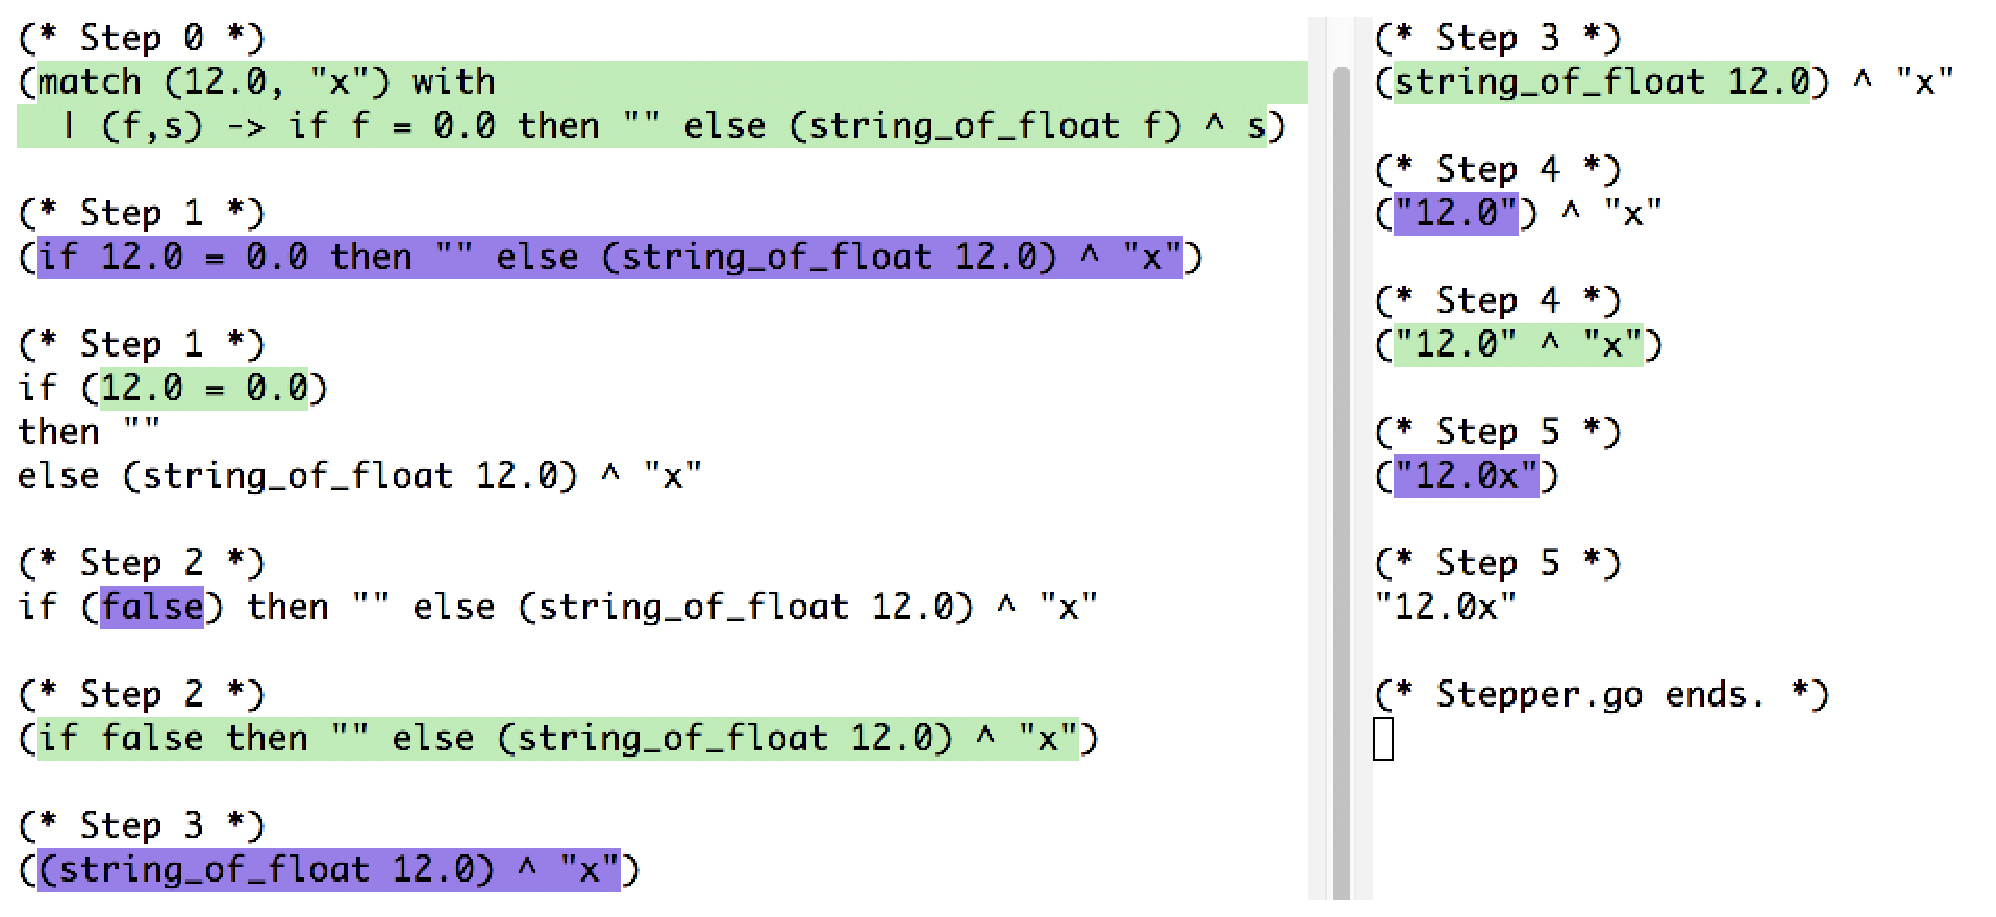
\includegraphics[width=14cm]{3/longexample.eps}
  \caption{Evaluating programs using the actual stepper}
  \label{figure:ocamlstep}
\end{figure}

\begin{figure}
  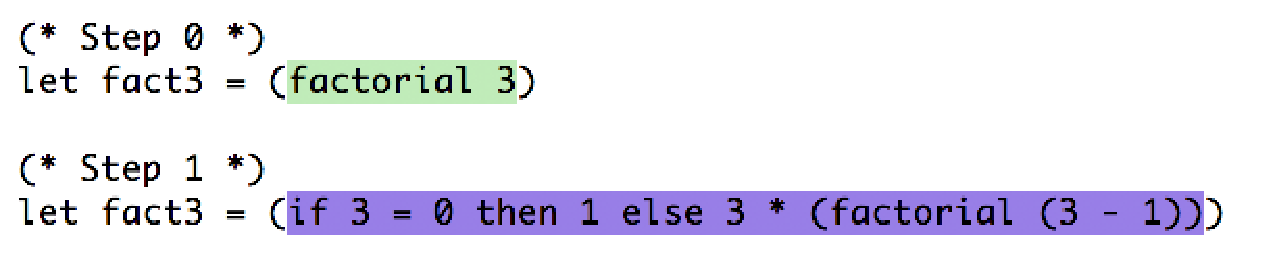
\includegraphics[width=10cm]{3/beforeskip.eps}
  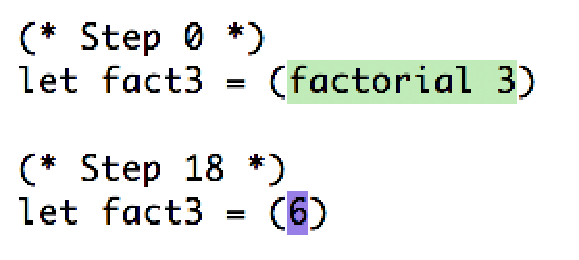
\includegraphics[width=4.3cm]{3/afterskip.eps}
  \caption{Skipping evaluation of the factorial function}
  \label{figure:factskip}
\end{figure}

To allow the user to adjust granularity of steps, we provide an option for skipping the evaluation of the current function application.  Let us look at Figure \ref{figure:factskip}, which shows skipping of the factorial function.  By pressing the ``skip'' button, we can directly go from the program on the left to the one on the right, without seeing the intermediate steps that appear during the evaluation of the function's body.  This feature helps us focus on the steps we are interested in, allowing us to grasp the overall flow of the execution.

The skipping feature requires some modifications to the \texttt{eval} function (Figure \ref{figure:skipapp}).  The idea is to sandwich the steps within an application between two strings: \texttt{(* Application n start *)} and \texttt{(* Application n end *)}.  Here, \texttt{n} tells us at which step we have entered the application.  These strings are printed using the \texttt{apply\_start} and \texttt{apply\_end} functions, and help the Emacs Lisp program to hide unnecessary steps.  We show an example output sequence in Figure \ref{figure:skipping}.


\begin{figure}
\begin{alltt}
let rec eval expr ctxt = match expr with
    ...
  | App (e1, e2) ->
    begin
      let v2 = eval e2 (add ctxt (CAppR e1)) in
      let v1 = eval e1 (add ctxt (CAppL v2)) in
      match v1 with
      | Lam (x, e) ->
        let e' = subst e x v2 in
        \colorbox{lightgray}{let apply_num = apply_start () in}                (* output start mark *)
        memo (App (v1, v2)) e' ctxt;
        let v = eval e' ctxt in
        \colorbox{lightgray}{apply_end apply_num;}                               (* output end mark *)
        v
      | _ -> failwith "not a function"
    end
  | ...
\end{alltt}
\caption{Skipping application}
\label{figure:skipapp}
\end{figure}

\begin{figure}
\texttt{(* Step 0 *) (f 4) + \colorbox{lightgreen}{10 * 100}\\
(* Step 1 *) (f 4) + \colorbox{purple}{1000}\\
(* Application 1 start *)\\
(* Step 1 *) \colorbox{lightgreen}{f 4} + 1000\\
(* Step 2 *) \colorbox{purple}{(4 * 2) - 1} + 1000\\
(* Step 2 *) \colorbox{lightgreen}{(4 * 2} - 1) + 1000\\
(* Step 3 *) \colorbox{purple}{(8} - 1) + 1000\\
(* Step 3 *) \colorbox{lightgreen}{8 - 1} + 1000\\
(* Step 4 *) \colorbox{purple}{7} + 1000\\
(* Application 1 end *)\\
(* Step 4 *) \colorbox{lightgreen}{7 + 1000}\\
(* Step 5 *) \colorbox{purple}{1007}}
\caption{Stepping application}
\label{figure:skipping}
\end{figure}
